\documentclass{article}
	
\usepackage{thesis_style}

\bibliographystyle{ieeetr}
\graphicspath{{./img/}}

\begin{document}
	\title{Event-Triggered Saturating Attitude Controller\\ \large Problem Statement}
	\author{Diogo Almeida}
	\maketitle	
	The following is a draft of the problems and proposed solutions for my thesis project, namely the control of a quadcopter attitude using event triggered strategies. It is proposed the implementation of a saturating controller that fully exploits the available control torques, together with a Lyapunov based event triggering function.
	
	\section{The attitude controller}
	
		Proposed by Fritsch, Henze and Lohmann in \cite{lohmann_attitude}, the attitude controller implements a control law that stabilizes a quadcopter attitude in two steps. Firstly, the thrust axis of the quad is aligned with the reference direction. Secondly, the yaw angle of the vehicle is corrected. The control variables here are the displacement angle of the thrust axis, $\varphi$, and the yaw error, $\vartheta$. Prioritizing the thrust axis direction has advantages if the primary concern of the higher level control revolves around the translational movement of the robot. Another advantage lies on the controller's hability to take advantage of the actuating power available by explicitly modelling the maximum torques the system can provide and exploiting that knowledge by saturating the control torques whenever possible. This is achieved by adopting an energy shaping approach, in which a desired energy for the system is designed and a damping strategy that penalizes movements that go against the reference equilibrium, while boosting the ones that go in the desired way, is applied. The resulting control torques are given by
		\begin{equation}
			\boldsymbol \tau \mathbf{(x)} = \mathbf{T(q)}-\mathbf{D(x)} \boldsymbol \omega\; ,
			\label{control}
		\end{equation}
		where $\mathbf{q}$ is the quaternion that represents the attitude error of the quadcopter, $\boldsymbol \omega = \left [\omega_x \;\; \omega_y \;\; \omega_z \right ]^\top$ are the angular velocities of the quad around its three body frame axis, $\mathbf{T(q)}$ is the torque field that the desired energy would generate and $\mathbf{D(x)}$ is a positive semi-definite damping matrix that allows for the control saturation as well as the almost global assymptotic stability of the controlled system. Finally, the state of the system with respect to the attitude is given by $\mathbf{x} = \left [ \mathbf{q} \;\; \boldsymbol \omega \right]^\top$. 

		The control law \eqref{control} is designed to ensure that a Lyapunov function (LF) consisting of the sum of the system kinectic energy and an artificial potential energy has a time derivative given by
		\begin{equation}
			-\boldsymbol \omega^\top \mathbf{D(x)} \boldsymbol \omega \leq 0.
			\label{control2}
		\end{equation}
		
		The authors of \cite{lohmann_attitude} were able to prove assymptotic stability based on LaSalle's Stability theorem. The baseline result for this controller, under the initial conditions in \cite{lohmann_attitude} are given in figure \ref{baseline}.
		\begin{figure}
			\centering
			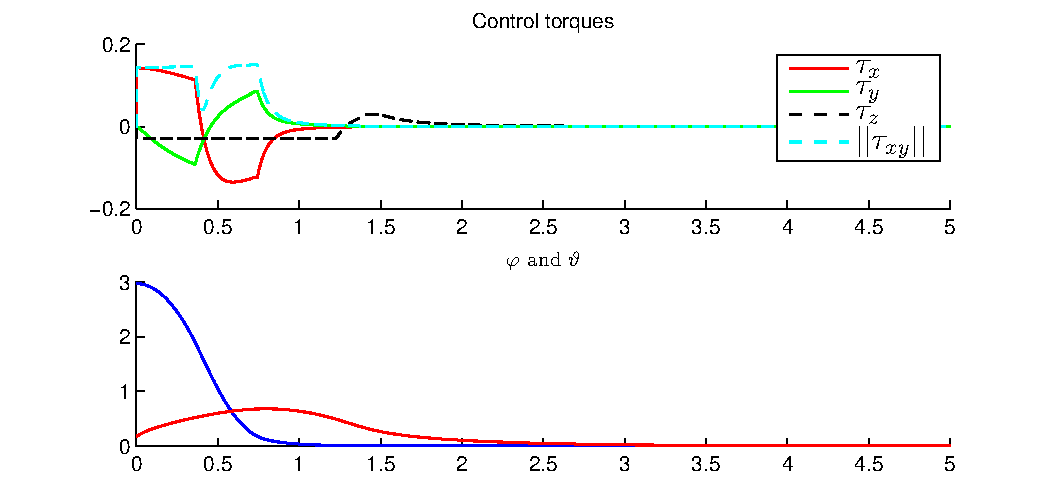
\includegraphics[width=\textwidth]{baseline}
			\caption{The applied torques and resulting behavior of the control variables for the saturating controller \cite{lohmann_attitude}\label{baseline}}
		\end{figure}
		
	\section{Event-triggered strategy}
		
		\subsection{Lyapunov based scheduling}
			The main problem in event-triggered implementations is to find an execution rule that allows to generate the sampling instants $t_k$ in such a way that the stabilization of the system is ensured, while avoiding accumulation points, that is, having the inter sampling time decreasing to zero. One systematic approach to the problem is given by \cite{tabuada_event_control}, where a sampling instant is generated every time the time derivative of the LF, $V(\mathbf{x})$, of the system violates an inequality condition. This strategy requires the LF to be bounded above and below by strictly increasing functions of the state and for its time derivative to be upper bounded by an 'error term' $-\alpha(|\mathbf{x}|) + \gamma(|\mathbf{e}|)$, where $\mathbf{e}$ is the difference between the state at the current time $t$ and at the last sampling instant $t_k$
			\begin{equation}
				\begin{array}{lll}
					\underline \alpha(|\mathbf{x}|) \leq & V(\mathbf{x}) & \leq \overline \alpha(|\mathbf{x}|) \\\\
					\, &\dot V(\mathbf{x}) &\leq -\alpha(|\mathbf{x}|) + \gamma(|\mathbf{e}|) \\
				\end{array}
				\label{event}
			\end{equation}
			and, by ensuring 
			\begin{equation}
				\gamma(|\mathbf{e}|) \leq \sigma \alpha(|\mathbf{x}|)\, , \;\; 0 < \sigma < 1
				\label{up_rule}
			\end{equation}
			we get $\dot V(\mathbf{x}) \leq 0$ at all times.
		
		\subsection{Threshold based scheduling}
			A simpler alternative to use as an execution rule is to define a threshold $\overline e$ for the difference between the control variable at the time $t_k$ \cite{lehmann}, \emph{i.e.} the last instant the control signal was updated, and the current value at the time $t$, over which the control signal is recomputed. However, it does not offer the guarantee that the system will remain stable when enforcing this update rule. As such, it probably needs to be tuned experimentally to obtain acceptable results without degrading performance too much.
			

	\section{Possible approaches}
		What follows are some ideas for event-triggering rules that can be implemented together with the saturating controller.
		
		\subsection{Lyapunov based Saturating Event Triggered control}
			This is the approach discussed in \cite{tabuada_event_control}. The event triggering rule is obtained from the time derivative of the LF of the controlled system, \eqref{control2}. For that, a $\alpha(|\mathbf{x}|)$ and $\gamma(|\mathbf{e}|)$ class-$\mathcal{K}$ functions need to be found that comply with \eqref{event} and allows for the definition of the update rule \eqref{up_rule}. Fritsch et al. \cite{lohmann_attitude} define $\mathbf{D(x)}$ as
			\begin{equation}
				\mathbf{D(x)} = \begin{bmatrix}
									\kappa_{xy}(\mathbf{x}) \mathbf{D}_{xy}(\mathbf{x}) &	\mathbf{0} \\
									\mathbf{0}	&	\kappa_z(\mathbf{x})d_z(\mathbf{x})\\
								\end{bmatrix}
				\label{D_mat}
			\end{equation}
			where
			\[
				\mathbf{D}_{xy}(\mathbf{x}) = \frac{d_\varphi(\mathbf{x})}{1-q_p^2} \begin{bmatrix}
																					q_x^2 & q_x q_y\\
																					q_x q_y & q_y^2
																				 \end{bmatrix}
																				 +
																				 \frac{d_\perp}{1-q_p^2} \begin{bmatrix}
																				 							q_y^2 & -q_x q_y \\
																				 							-q_x q_y & q_x^2
																				 						 \end{bmatrix}
		  \]
		  \begin{comment}
			 hence, we obtain
			 \[
			 	\mathbf{D(x)} = \begin{bmatrix}
			 	 					\kappa_{xy}(\mathbf{x})\frac{d_\varphi(\mathbf{x}) q_x^2 + d_\perp q_y^2}{1-q_p^2} & \kappa_{xy}(\mathbf{x})\frac{q_x q_y(d_\varphi(\mathbf{x})-d_\perp)}{1-q_p^2} & 0 \\
			 	 					\kappa_{xy}(\mathbf{x})\frac{q_x q_y(d_\varphi(\mathbf{x})-d_\perp)}{1-q_p^2} & \kappa_{xy}(\mathbf{x})\frac{d_\varphi(\mathbf{x}) q_y^2 + d_\perp q_x^2}{1-q_p^2} &  0 \\
									0 & 0	&	\kappa_z(\mathbf{x})d_z(\mathbf{x})\\
								\end{bmatrix}
			\]
		\end{comment}
		hence, the time derivative of the LF, \eqref{control2} becomes
		\begin{equation}
			-\frac{\kappa_{xy}(\mathbf{x})}{1-q_p^2} \left [ \omega_x^2 \left (d_\varphi(\mathbf{x}) q_x^2 + d_\perp q_y^2 \right ) + \omega_y^2 \left (d_\varphi(\mathbf{x}) q_y^2 + d_\perp q_x^2 \right ) \right ] - \omega_z^2 \kappa_z(\mathbf{x}) d_z(\mathbf{x}).
			\label{v_dot}
		\end{equation}
		
		One can easily see that, since in the equilibrium $q_p = \pm 1$ and, by multiplying the first element in the sum \eqref{v_dot} by $1-q_p^2$, we obtain a function that is always bigger than \eqref{v_dot}. That can be used to find the event rule \eqref{up_rule} while ensuring $\dot V(\mathbf{x}) \leq 0$ for all $\mathbf{x}$ different than $\mathbf{0}$.
		
		\subsection{Heuristic approach}
			Another alternative is to discard altogether the Lyapunov based approach and to generate an event-triggering mechanism based on either the state error as defined above, or the error with respect to the reference. In the first case, the control signal is updated every time the state deviates more than a certain value from the state at the previous sampling time \cite{lehmann}. In the second case, one can do periodic sampling when outside a 'tolerance region' specified by the system designer \cite{astrom}. Moreover, if the purpose of the event triggering system is to save network resources, as in \cite{lehmann}, the control algorithm may run periodically over an input error that is updated according to the update rule, or the control algorithm may be the limited to run only at event times, and the control signal is kept constant in the meanwhile. All these approaches lack stability results \emph{a priori} and require an analysis case by case.
		
	\section{Lyapunov based event triggering results}
		Given a controller that stabilizes the system, if we fulfil the conditions in \cite[Theorem~3.1]{tabuada_event_control}, we can get a control update rule that preserves the stability of the system and does not pose the risk of accumulation points. The main problem with this approach is that it is not easy to find an $\alpha{(|\mathbf{x}|)}$ that is stricly increasing and satisfies the inequality. Remembering that a desired equilibrium has two corresponding points in the quaternion space, $\boldsymbol \omega = \mathbf{0}$ and $\mathbf{q} = \left [0 \;\; 0 \;\; 0 \;\; \pm 1 \right ]$, we have that 
		\begin{equation}
			\alpha(\mathbf{x}) = -\boldsymbol \omega^\top D_\alpha(\mathbf{x}) \boldsymbol \omega
			\label{alpha}
		\end{equation}
		where
		\[
			D_\alpha(\mathbf{x}) = \begin{bmatrix}
									\kappa_{xy}(\mathbf{x}) (1-q_p^2)\mathbf{D}_{xy}(\mathbf{x}) &	\mathbf{0} \\
									\mathbf{0}	&	\kappa_z(\mathbf{x})d_z(\mathbf{x})\\
								  \end{bmatrix}
		\]
		satisfies \eqref{event}, though it is not a class-$\mathcal{K}$ function, nor a function of the norm of the state. The need for the function to be strictly increasing with the norm of the state is to ensure that there are no accumulation points. This can be solved by imposing a minimum inter sampling time\footnote{But will that grant stability?}. The stability of the resulting system is ensured by \eqref{up_rule}. Indeed, the implementation of the update rule with $\alpha(\mathbf{x})$, as defined in \eqref{alpha}, allows for the convergence of the controlled variables without any noticeable performance issues, see figure \ref{event_results1} for the results with $\sigma = 0.9$.
		\begin{figure}[ht]
			\centering
			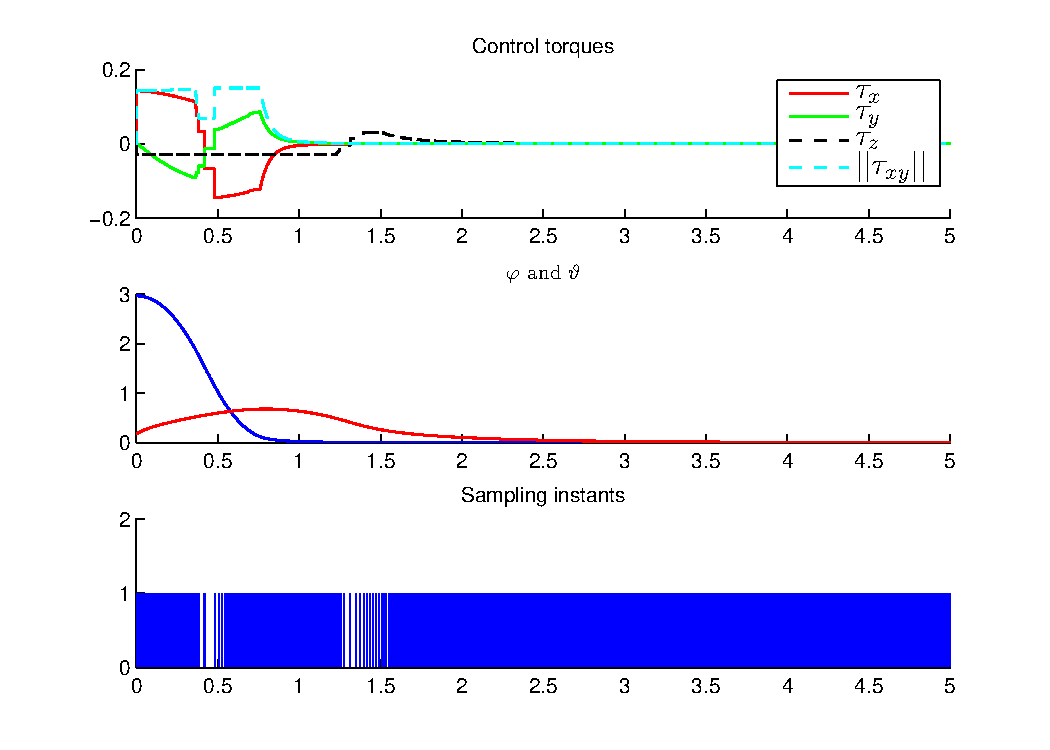
\includegraphics[width=\textwidth]{event_1}
			\caption{Results using the update rule \eqref{up_rule} with $\alpha(\mathbf{x})$ defined as in \eqref{alpha} \label{event_results1}}
		\end{figure}
		
		\subsection{How to deal with accumulation points}
			The main problem with this result, is the decrease in the inter-sampling time as the simulation goes on. Eventually, when the state of the system stabilizes, inter-sampling time coincides with the sampling time used for the simulations. It seems as if $\gamma(|\mathbf{e}|)$ is decreasing slower than $\alpha(\mathbf{x})$, and this results in the inequality \eqref{up_rule} being violated every time it is checked. I assume this is a direct consequence of not enforcing $\alpha(\mathbf{x}) \in \mathcal{K}$. My proposal is to add a very small $\epsilon_{x}$ to \eqref{up_rule} so as to become
		\begin{equation}
			\gamma(|\mathbf{e}|) \leq \sigma \alpha(|\mathbf{x}|) + \epsilon_x\, , \;\; 0 < \sigma < 1.
			\label{up_rule2}
		\end{equation}
		
		With this new update rule we introduce a dead zone for the state-error that may yield stability problems, but at the same time allows for the inter-sampling time to grow unbounded if the state is in the desired equilibrium, see figure \ref{event_results2} with $\sigma = 0.9$ and $\epsilon_x = 0.05$.
		\begin{figure}
			\centering
			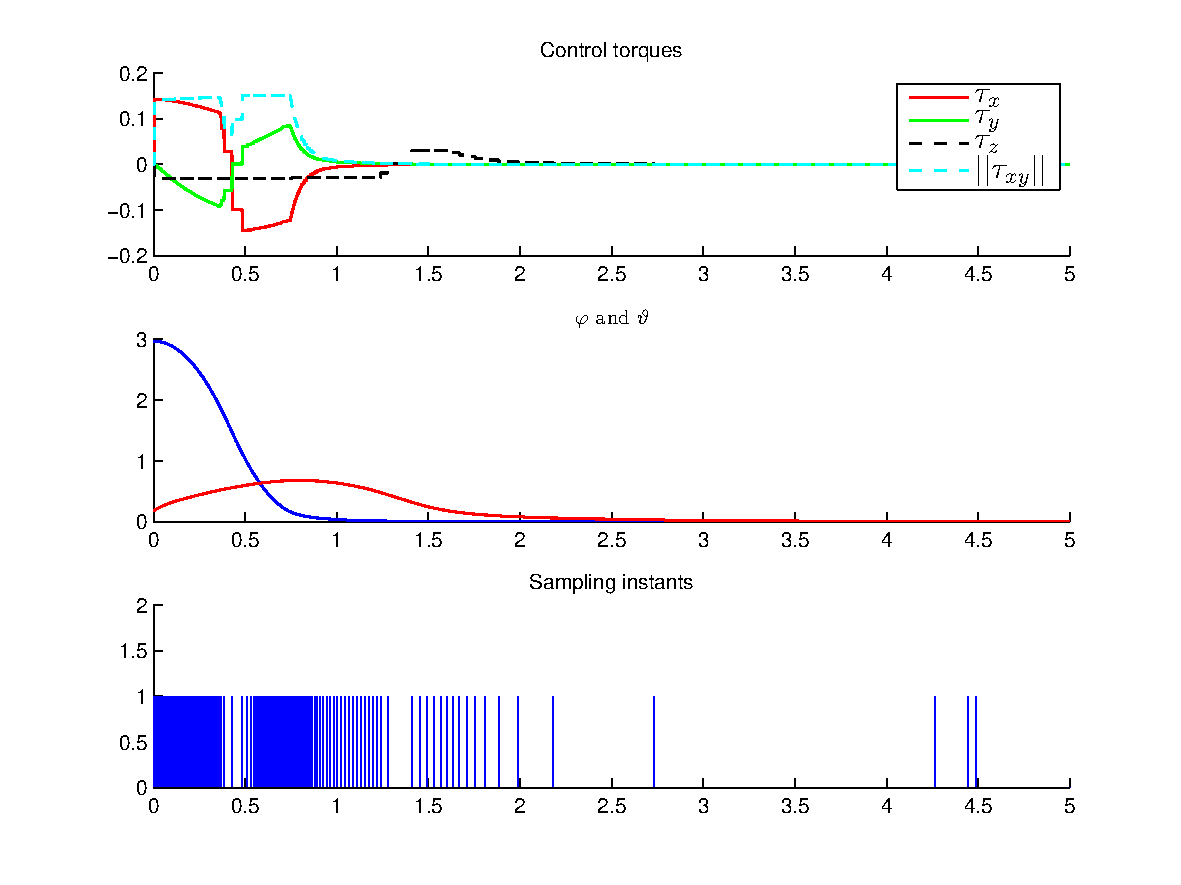
\includegraphics[width=\linewidth]{event_2}
			\caption{Results for the execution rule \eqref{up_rule2}\label{event_results2}}
		\end{figure}
		
	\section{Error based methods}
		Besides tying the event triggering to the evolution of the time derivative of the LF of the system, one can try to implement rules based purely on the state error, that is, on how much the state has changed since the last time the control was updated or even by defining an area of admissible error, where the control is kept constant while the state of the system remains inside it.
		\subsection{State error method}
			Here, the update rule is based on the evolution of the state since the last time the control was updated. Given the error
			\[
				\mathbf{e} = \mathbf{x}(t_k) - \mathbf{x}(t),
			\]
			the control is updated every time the norm of the state error grows beyond a certain threshold
			\begin{equation}
				|\mathbf{e}| > \sigma_e.
				\label{up_rule3}
			\end{equation}
			
			One advantage of this rule relies on its simplicity. If the state is diverging too much from the one we had the last time the control was updated, then it is time to do it again. Stability may be a concern here, at least when near the equilibrium, the control may be so agressive that the state doesn't stay where it is meant to be, resulting in poor performance and extra control updates. The value of the threshold $\sigma_e$ impacts the results significantly as well. For $\sigma_e=0.1$ the observed results are the ones in figure \ref{event_results3}.
			\begin{figure}
				\centering
				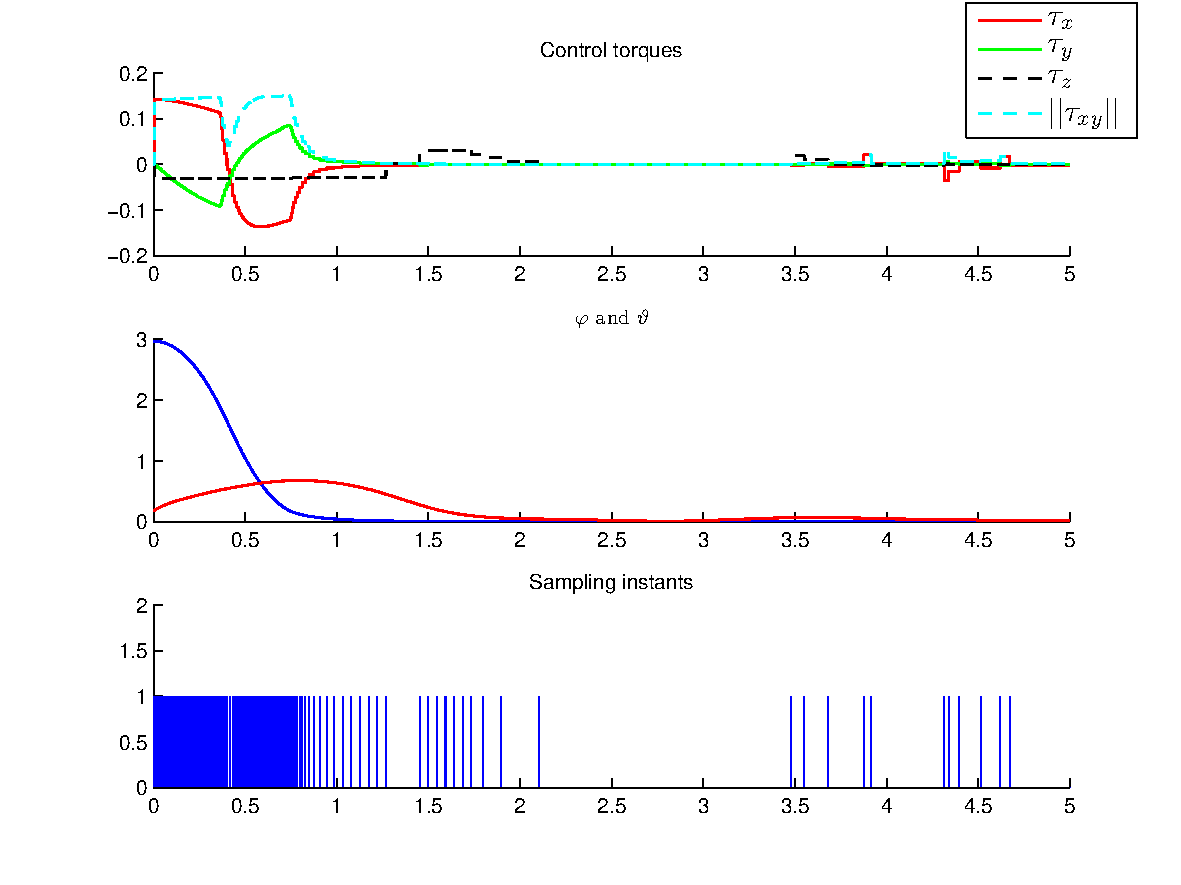
\includegraphics[width=\textwidth]{event_3}
				\caption{Results for the execution rule \eqref{up_rule3} \label{event_results3}}
			\end{figure}
			With this threshold value, it is noticeable that the controller lets the state move away from the desired equilibrium and reacts later in the simulation to correct it. This results in a diverging behavior of the state when it should be resting in the reference value (figure \ref{event_details1}).
			\begin{figure}
				\centering
				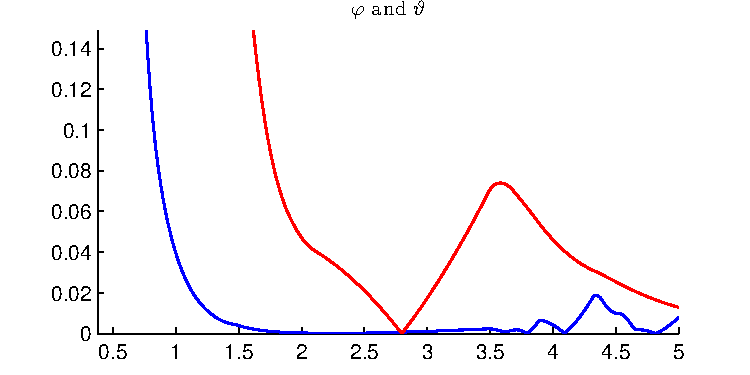
\includegraphics[width=0.7\textwidth]{event_detail1}
				\caption{Details of the diverging behavior when using execution rule \eqref{up_rule3} \label{event_details1}}
			\end{figure}
			A similar behavior is observed when using the rule \eqref{up_rule2} for larger values of $\sigma_e$, case where there are less updates to the control signal, but results in larger tolerance for positive $\dot V(\mathbf{x})$. 
		\subsection{Error with respect to the reference}
			Another simple idea is to update the control value every time the state leaves an admissible set \cite{astrom}. This is similar to having a relay in the control loop that closes the feedback loop only when the error grows above a certain threshold. Here, the error may be given as
			\[
				\mathbf{e} = \mathbf{x}(t) - \mathbf{x}_{d},
			\]
			where $\mathbf{x}_d$ is the state in the equilibrium. Since the proposed controller works on the error between the current state and the reference, the desired equilibrium is always the same, which makes it easy to implement the update rule. In figure \ref{event_results4} are depicted the results for an admissible deviation of $1$ percent of the state norm.
			\begin{figure}
				\centering
				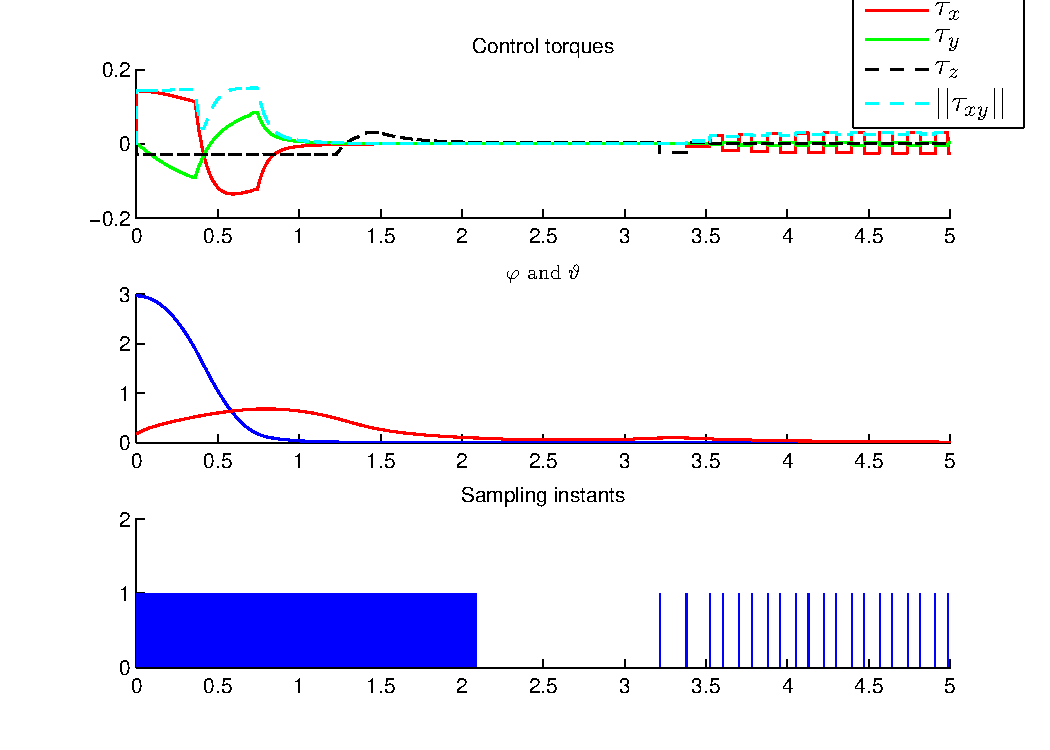
\includegraphics[width=\textwidth]{event_4}
				\caption{Results for the admissible set rule\label{event_results4}}
			\end{figure}
			For every value of the admissible error experimented with, the oscillating behavior appeared, sooner or later. That seems reasonable, since the system is unstable while in open-loop. Changing the error value has an impact in the overall performance of the system while near the equilibrium, as well as on the number of control updates while near the admissible set.
			
	\section{Comparison between approaches}
		With the exception of the update rule \eqref{up_rule}\footnote{Or even with the inclusion of the update rule \eqref{up_rule}. Is the Lyapunov based analysis \eqref{event} only valid for continuous systems? }, all the approaches analysed here do not ensure that the assimptotic stability of the system is preserved. That may be acceptable or lead to unwanted behavior. There may be a tradeoff between performance and number of time events. Finally, some techniques may be objectively better than others in some aspects. Some comparison rules are proposed to benchmark the event rules.
		\subsection{Number of updates}
			The trivial measurement of performance is the number of updates of the control signal during the same time period. Less updates means that the control algorithm is called less often, resulting in computational savings. The simulation results for the cases above are presented in table \ref{tab:ticks}.
			\begin{table}[ht]
				\centering
				\begin{tabular}{|c|l|}
					\hline
					Strategy & Updates \\
					\hline
					Baseline & $5000$ \\
					\hline
					Rule \eqref{up_rule} & $2801$ $(56 \%)$ \\
					\hline
					Rule \eqref{up_rule2} & $439$ $(9 \%)$ \\
					\hline
					Rule \eqref{up_rule3} & $155$ $(3 \%)$ \\
					\hline
					Admissible set rule & $2109$ $(42 \%)$\\
					\hline
				\end{tabular}
				\caption{Number of control updates}
				\label{tab:ticks}
			\end{table}
		
		\subsection{Control signal energy}
			One of the purposes of using event-triggered control is to reduce the energy consumption of the overal system, by minimizing the CPU usage. Those gains may be lost if the resulting control signals uses more energy, defined as
			\[
				E_i = \frac{1}{T}\sum_{t_k=0}^T \tau_i^2\;\;\; , \; i=\left \{x,y,z \right \}.
			\]
			
			The respective results are presented in table \ref{tab:energy}.
			\begin{table}[ht]
				\centering
				\begin{tabular}{|c|l|l|l|}
					\hline
					Strategy & $\tau_x$ & $\tau_y$ & $\tau_z$ \\
					\hline
					Baseline & $2.3333$ & $0.53697$ & $0.25928$ \\
					\hline
					Rule \eqref{up_rule} & $2.4573$ $(105 \%)$ & $0.5833$ $( 109\%)$ & $0.26245$ $( 101\%)$  \\
					\hline
					Rule \eqref{up_rule2} & $2.477$ $(106 \%)$ & $0.60163$ $(112 \%)$ & $0.26369$ $(102 \%)$ \\
					\hline
					Rule \eqref{up_rule3} & $2.3949$ $(102 \%)$ & $0.54307$ $( 101\%)$ & $0.29017$ $( 112 \%)$ \\
					\hline
					Admissible set rule & $2.539$ $(108 \%)$ & $0.54029$ $(101 \%)$ & $0.28066$ $( 108\%)$\\
					\hline
				\end{tabular}
				\caption{Torques energy}
				\label{tab:energy}
			\end{table}
	
	\section{Work plan}
		The parameters used for each approach were not tuned to obtain the best results. This may have a significant impact in the comparisons that were made. There may be worth it to look deeply into the definition of \eqref{D_mat} to try to find a better $\alpha(\mathbf{x})$ function, or even one that fulfills the theorems in \cite{tabuada_event_control}. Furthermore, these approaches are only applied in simulations where I assume full access to the system state. Another issue concerns the implementation. Getting to know the system and the low level control code that is already implemented in the Arducopter may take some time. There is a need to estimate the maximum available torques that the system can output, to ensure that the proposed controller will behave properly. Finally, setting up a systematic way of testing and comparing these approaches in the real system is something that is important to do. A possible approach to the project is listed bellow:
		\begin{itemize}
			\item Get to know the system: where is the current attitude control implemented; how and where in the code is the state being measured/estimated; how does the embedded controller in the quad communicates with an external computer over the motes.
			\item Implement a framework that can be used to test attitude controllers and to benchmark them: set a program that allows to measure and process data required for the analysis of the controllers and event-triggering techniques.
			\item Assemble an experimental setup that ensures that multiple tests can be carried away in the same conditions, for example, by only allowing one degree of freedom of the quad to be available at any time.
			\item Depending on how to work goes on, iterate between experimental and theoretical work to try and cover a good array of event-triggering techniques.
		\end{itemize}
	
	
	\bibliography{thesis_bib}
\end{document}
